\documentclass{beamer}
\mode<presentation>
\usepackage{amsmath}
\usepackage{amssymb}
%\usepackage{advdate}
\usepackage{adjustbox}
\usepackage{subcaption}
\usepackage{enumitem}
\usepackage{multicol}
\usepackage{mathtools}
\usepackage{listings}
\usepackage{url}
\def\UrlBreaks{\do\/\do-}
\usetheme{Boadilla}
\usecolortheme{lily}
\setbeamertemplate{footline}
{
  \leavevmode%
  \hbox{%
  \begin{beamercolorbox}[wd=\paperwidth,ht=2.25ex,dp=1ex,right]{author in head/foot}%
    \insertframenumber{} / \inserttotalframenumber\hspace*{2ex} 
  \end{beamercolorbox}}%
  \vskip0pt%
}
\setbeamertemplate{navigation symbols}{}

\providecommand{\nCr}[2]{\,^{#1}C_{#2}} % nCr
\providecommand{\nPr}[2]{\,^{#1}P_{#2}} % nPr
\providecommand{\mbf}{\mathbf}
\providecommand{\pr}[1]{\ensuremath{\Pr\left(#1\right)}}
\providecommand{\qfunc}[1]{\ensuremath{Q\left(#1\right)}}
\providecommand{\sbrak}[1]{\ensuremath{{}\left[#1\right]}}
\providecommand{\lsbrak}[1]{\ensuremath{{}\left[#1\right.}}
\providecommand{\rsbrak}[1]{\ensuremath{{}\left.#1\right]}}
\providecommand{\brak}[1]{\ensuremath{\left(#1\right)}}
\providecommand{\lbrak}[1]{\ensuremath{\left(#1\right.}}
\providecommand{\rbrak}[1]{\ensuremath{\left.#1\right)}}
\providecommand{\cbrak}[1]{\ensuremath{\left\{#1\right\}}}
\providecommand{\lcbrak}[1]{\ensuremath{\left\{#1\right.}}
\providecommand{\rcbrak}[1]{\ensuremath{\left.#1\right\}}}
\theoremstyle{remark}
\newtheorem{rem}{Remark}
\newcommand{\sgn}{\mathop{\mathrm{sgn}}}
\providecommand{\abs}[1]{\left\vert#1\right\vert}
\providecommand{\res}[1]{\Res\displaylimits_{#1}} 
\providecommand{\norm}[1]{\lVert#1\rVert}
\providecommand{\mtx}[1]{\mathbf{#1}}
\providecommand{\mean}[1]{E\left[ #1 \right]}
\providecommand{\fourier}{\overset{\mathcal{F}}{ \rightleftharpoons}}
%\providecommand{\hilbert}{\overset{\mathcal{H}}{ \rightleftharpoons}}
\providecommand{\system}{\overset{\mathcal{H}}{ \longleftrightarrow}}
	%\newcommand{\solution}[2]{\textbf{Solution:}{#1}}
%\newcommand{\solution}{\noindent \textbf{Solution: }}
\providecommand{\dec}[2]{\ensuremath{\overset{#1}{\underset{#2}{\gtrless}}}}
\newcommand{\myvec}[1]{\ensuremath{\begin{pmatrix}#1\end{pmatrix}}}
\let\vec\mathbf

\lstset{
%language=C,
frame=single, 
breaklines=true,
columns=fullflexible
}

\numberwithin{equation}{section}

\title{12.9.4.9}
\author{Dhawal \\ ee24btech11015,\\IIT Hyderabad.}

\date{\today} 
\begin{document}

\begin{frame}
\titlepage
\end{frame}

\section*{Outline}
\begin{frame}
\tableofcontents
\end{frame}
\section{Problem}
\begin{frame}
\frametitle{Problem Statement}
%
 Find the solution of the differential equation $\frac{dy}{dx}=\sin^{-1}{x}$.

\end{frame}

%\subsection{Literature}
\section{Solution}
\subsection{Theoretical Solution}
\begin{frame}
\frametitle{Theoretical Solution}
%\framesubtitle{Literature}
Using the given D.E. , we get,
\begin{align}
    \frac{dy}{dx} &= \sin^{-1}{x}
\end{align}

Integrate both sides with respect to $x$:
\begin{align}
y &= \int \sin^{-1}{x} \; dx
\end{align}

Using integration by parts:
\begin{align}
\int u \, dv &= uv - \int v \, du
\end{align}
Let:
\begin{align}
u = \sin^{-1}{x}, \;  dv = dx
\end{align}
Then:
\begin{align}
du = \frac{1}{\sqrt{1-x^2}} \, dx, \; v = x
\end{align}

\end{frame}
\begin{frame}
\frametitle{Theoretical Solution}
Substituting into the integration by parts formula:
\begin{align}
\int \sin^{-1}{x} \, dx &= x \sin^{-1}{x} - \int x \frac{1}{\sqrt{1-x^2}} \, dx
\end{align}

For the remaining integral, let $ u = 1 - x^2 $, so $ du = -2x \, dx $:
\begin{align}
\int x \frac{1}{\sqrt{1-x^2}} \, dx &= -\frac{1}{2} \int \frac{1}{\sqrt{u}} \, du \\
&= -\sqrt{u} + C \\
&= -\sqrt{1-x^2} + C
\end{align}

Thus, the solution to the differential equation is:
\begin{align}
y = x \sin^{-1}{x} + \sqrt{1-x^2} + C
\end{align}
\end{frame}
\subsection{Euler Formula}
\begin{frame}
\frametitle{Euler Formula}

Using a classical definition of derivative, we get,\\
\begin{align}
    f^{\prime}\brak{x} &= \frac{f\brak{x+h}-f\brak{x}}{h}\\
    \implies f\brak{x+h} &= f\brak{x} + h f^{\prime}\brak{x}
\end{align}
By increasing $x$ n each iteration by $h$ and let $C=0$, we are getting $y$ by,
\begin{align}
x_0 &= 0\\
y_0 &= 1\\
h &= 0.01\\
n &= 100
\end{align}
Using Euler Method, we get difference equation,
\begin{align}
y_{n+1} &= y_n + h\frac{dy}{dx}\Big|_{\brak{x_n,y_n}}\\
y_{n+1} &= y_n + h\sin^{-1}{x_n}
\end{align}


\end{frame}

\subsection{Bilinear transfrom}
\begin{frame}
\frametitle{Bilinear transfrom}

\begin{align}
    \frac{dy}{dx} &= \sin^{-1}{x}
\end{align}
Taking Laplase of $\frac{dy}{dx}$ and putting $\sin^{-1}{x}$ as $F\brak{s}$
\begin{align}
    sY\brak{s}&=F\brak{s}\\
    \frac{Y\brak{s}}{F\brak{s}}&=\frac{1}{s}=H\brak{s}
\end{align}
Now, convert it into Z-transform
\begin{align}
    Y\brak{z}&=\frac{h}{2}\frac{1+z^{-1}}{1-z^{-1}}F\brak{z}\\
    Y\brak{z}\brak{1-z^{-1}}&=\frac{h}{2}\brak{1+z^{-1}}F\brak{z}
\end{align}
Applying inverse Z-transform, we get
\begin{align}
    y_{n}-y_{n-1}&=\frac{h}{2}\brak{\sin^{-1}{x_n}+\sin^{-1}{x_{n-1}}}
\end{align}

\end{frame}
\subsection{PLot}
\begin{frame}[fragile]
\frametitle{Plot}

\begin{figure}[h]
    \centering
    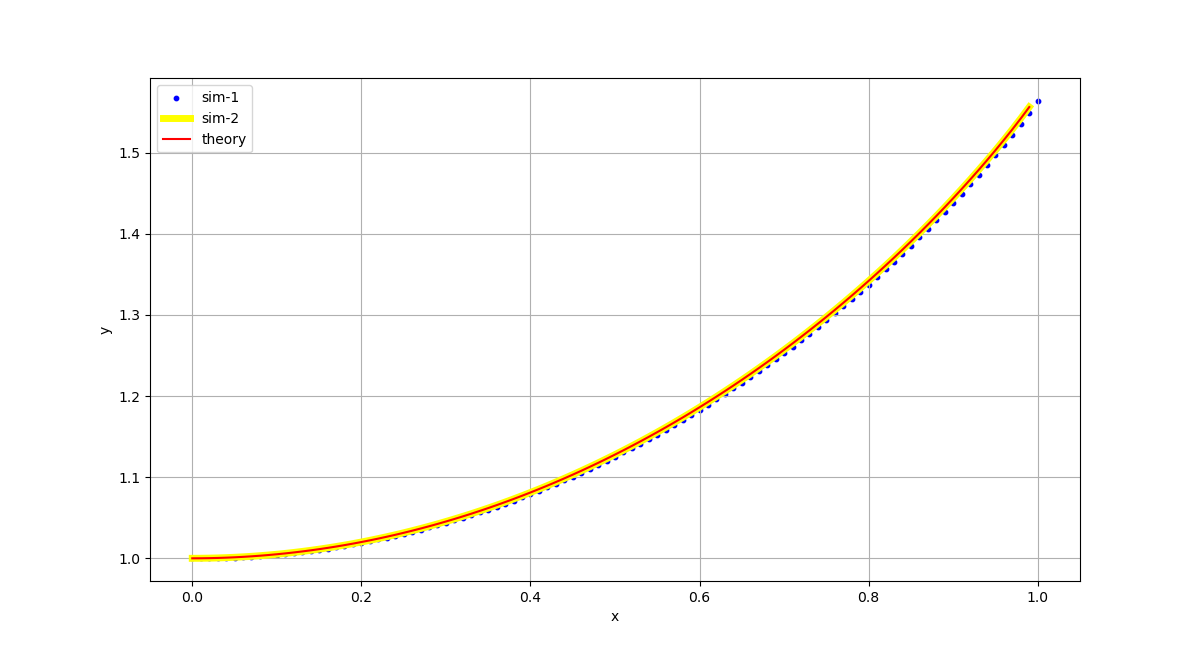
\includegraphics[width=\columnwidth]{figs/Figure_1.png}
    \caption{Plot of the differential equation }
    \label{fig:Plot}
    \end{figure}
\end{frame}

\section{Codes}
\begin{frame}[fragile]
\frametitle{Codes}
\begin{lstlisting}[language=C]
https://github.com/Dhawal24112006/EE1003/tree/main/NCERT/Q3/codes
    \end{lstlisting}
\end{frame}


\end{document}
